\section{Virtualizzatore}
Un virtualizzatore è un software che si occupa di astrarre le risorse hardware di un computer/server, facendo da intermediario tra esse e il software che deve girarci sopra. Astraendo le risorse, è possibile distribuirle in maniera agile e ottimizzata tra i vari software che le richiedono.
In ambito di virtualizzazioni server, la situazione più comune è la seguente: sulla macchina fisica è installato un \texttt{hypervisor}, che crea, gestisce e assegna risorse alle macchine virtuali, su cui viene installato un sistema operativo completo; sono poi queste macchine virtuali a offrire effettivamente i servizi.

\subsection{Caratteristiche e funzionamento}
Gli hypervisor rendono la virtualizzazione possibile attraverso una traduzione delle richieste tra le risorse fisiche e quelle virtuali.

Fondamentalmente, ci sono due tipi di hypervisor: quelli detti \texttt{bare-metal}, che vengono eseguiti direttamente sull'hardware fisico e sono spesso installati allo stesso livello del BIOS sulla scheda madre, e quelli detti \texttt{in-hosting}, che girano come software standard sul sistema operativo installato sull'hardware fisico (detto host system). Suddividendo le risorse, è possibile assegnarle non più a una sola macchina, ma a molteplici macchine virtuali.

Lo svantaggio degli hypervisor in-hosting è la loro maggiore latenza rispetto agli hypervisor bare-metal. Ciò è dovuto al fatto che la comunicazione tra hardware e hypervisor non è diretta, ma deve passare attraverso il sistema operativo che lo ospita. Questo tipo di hypervisor è anche detto client hypervisor, essendo più comunemente utilizzato da utenti finali e per il testing di software, scenari in cui la latenza non è particolarmente rilevante.

\begin{figure}[ht]
    \centering
    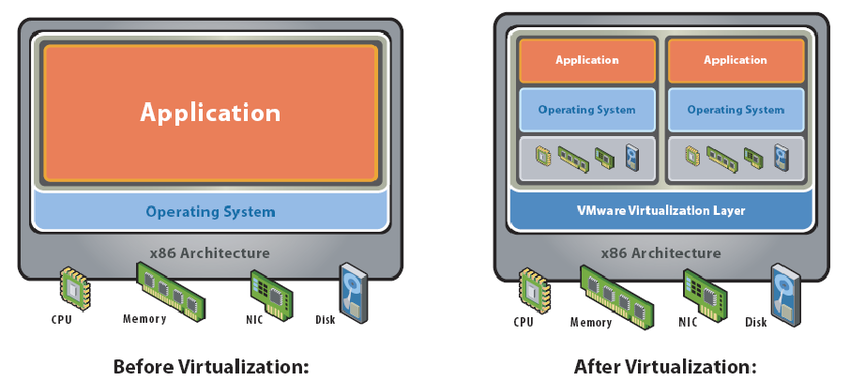
\includegraphics[width=10cm]{figure/virtualization.png}
    \caption{Installazione fisica vs Installazione virtuale}
\end{figure}

\subsection{VirtualBox}
Durante le prime fasi di testing, abbiamo utilizzato Oracle VirtualBox \cite{virtualbox} sui nostri PC per creare un ambiente di simulazione. VirtualBox è un client hypervisor, open source e disponibile per tutti i sistemi operativi.
\subsection{VMWare ESXi}
Nella fase di realizzazione, abbiamo invece utilizzato un server reale, su cui era installato l'hypervisor VMWare ESXi \cite{esxi}. Una volta allocate le risorse necessarie, abbiamo installato CentOS 7 come sistema operativo sulla macchina virtuale come da requisito.
Questa macchina virtuale corrisponde al router/firewall nel diagramma di rete presentato nei capitoli precedenti.

\subsection{Installazione e configurazione dei servizi VPN}
Dopo una fase iniziale di configurazione dei servizi interni ed esterni illustrati nei requisiti, si è passati all'installazione e configurazione dei tre servizi VPN scelti per il testing.

\section{Installazione e configurazione di IPSec - tunnel mode}
Il primo servizio che è stato installato è IPSec, grazie all'implementazione open source offerta da strongSwan \cite{strongSwan}.


\subsection{Aggiunta dell'interfaccia di rete virtuale}
Prima di installare strongSwan, è necessario predisporre l'interfaccia di rete virtuale che verrà utilizzata per la creazione del tunnel VPN. Per fare ciò, è necessario abilitare le interfacce virtuali con il comando \texttt{modprobe dummy}.
A questo punto è possibile aggiungerla e configurarla, assegnandole:
\begin{itemize}
    \item un nome (e.g.: \texttt{strongswan0})
    \item un MAC Address qualunque - a patto che sia diverso da tutti quelli presenti nella subnet (e.g.: \texttt{C8:D7:4A:4E:47:50}),
    \item un indirizzo IP con la relativa maschera (e.g.: \texttt{10.0.2.1/24})
\end{itemize}
e abilitarla.

Una volta completato il tutto, visualizziamo il risultato con il seguente comando:
\begin{figure}[ht]
    \centering
    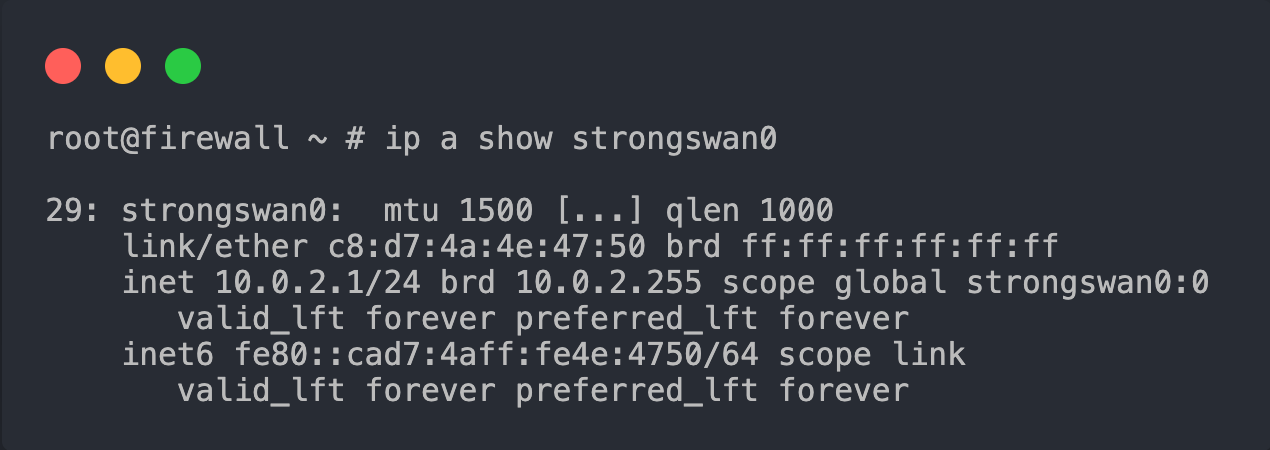
\includegraphics[width=10cm]{figure/show_sw0.png}
    \caption{Dettagli interfaccia virtuale strongswan0}
\end{figure}

\subsection{Installazione di strongSwan}
Per installare il daemon di strongSwan è sufficiente lanciare il comando \texttt{dnf install strongswan}, che si occuperà di scaricare e installare la versione più recente disponibile.

\subsection{Configurazione di strongSwan}
Per adattare il comportamento del servizio alle proprie esigenze, è necessario modificare il file di configurazione del servizio, che nel caso di strongSwan si trova nella directory \texttt{/etc/strongswan/}.
Al suo interno, andremo a inserire i parametri adatti. Di particolare rilievo sono i seguenti:

\begin{verbatim}

conn strongswanVPN      # per la connessione di nome strongswan VPN
    type=tunnel         # IPSec in tunnel mode
    keyexchange=ikev2   # Protocollo per lo scambio chiavi

    # Algoritmi di cifratura consentiti
    ike=aes256-sha256-modp2048,[...],aes256gcm16-prfsha512-ecp384!
    esp=aes256-sha256-modp2048,[...],aes256gcm16-ecp384!
    
    leftcert=server.crt # Certificato del server
    rightauth=eap-tls   # Protocollo di autenticazione
    rightdns=8.8.8.8    # DNS Server per il client

    # Range di indirizzi IP assegnabili ai client
    rightsourceip=10.0.2.10-10.0.2.100
\end{verbatim}

\subsection{Creazione del certificato per un client}
Una volta terminata la configurazione lato server, è necessario creare un certificato per ogni client che vorrà connettersi alla VPN. È possibile farlo tramite le funzioni della libreria OpenSSL. Essendo in ambiente di testing e non di produzione, non ci si è preoccupati di acquistare un certificato che abbia possibilità di firmare altri certificati; si è scelto infatti di utilizzare sempre OpenSSL per creare una Certificate Authority locale. Questo ha lo svantaggio che i client non hanno modo di verificare presso un ente stabilito (e.g.: Let's Encrypt, o altre CA affermate) la validità del certificato, ma il funzionamento è identico.

\section{Installazione e configurazione di OpenVPN over TCP}
Per il servizio OpenVPN, si è deciso di utilizzare la porta 443 TCP per testare le performance nel caso di reti con firewall stringenti.

\subsection{Installazione di OpenVPN}
L'installazione avviene tramite il comando \texttt{dnf install openvpn}, che scarica e installa tutto il necessario per eseguire il servizio.
Al file di configurazione di OpenVPN, sono state apportate alcune modifiche. Quelle più rilevanti sono le seguenti:

\begin{verbatim}
    port 1194, proto tcp    # Porta e procotollo da utilizzare
    
    # Dopo l'avvio, si disabilitino i privilegi di root
    user nobody, group nobody   

    # Rende la VPN una sottorete, con prefisso e maschera
    topology subnet         
    server 10.8.0.0 255.255.255.0

    push "dhcp-option DNS 8.8.8.8"   # DNS primario per i clients
    push "dhcp-option DNS 8.8.4.4"   # DNS secondario per i clients

    # Comunica ai client di far passare il loro traffico 
    #     attraverso il server VPN
    push "redirect-gateway def1 bypass-dhcp"   

    # Nomi dei file della CA, del certificato pubblico del server 
    #     e della relativa chiave privata
    ca ca.crt
    cert server_jH2NKwoak6pDEBoQ.crt
    key server_jH2NKwoak6pDEBoQ.key
    
    cipher AES-128-GCM  # Algoritmo scelto per la cifratura del canale

    tls-version-min 1.2 # Versione minima di TLS
    tls-crypt tls-crypt.key
    tls-cipher TLS-ECDHE-ECDSA-WITH-AES-128-GCM-SHA256  
\end{verbatim}

\subsection{Certificati}
Per la creazione della Certificate Authority e di tutti i certificati, sono state utilizzate le funzioni della libreria EasyRSA, messa a disposizione sulla repository GitHub di OpenVPN stesso.

\subsection{Configurazione del profilo VPN per un client}
Affinché un client possa connettersi alla VPN, è necessario che egli sia in possesso di un profilo contenente tutti i dettagli tecnici necessari a instaurare una connessione corretta con il server, e il suo certificato personale. In particolare, devono combaciare porta e protocollo utilizzato, gli algoritmi di cifratura, le funzioni di \emph{digest} e i parametri per TLS.

\section{Installazione e configurazione WireGuard}
L'installazione di WireGuard si effettua semplicemente con il comando \texttt{dnf install wireguard}, che si generi la chiave del server e che si inserisca all'interno del file di configurazione, insieme all'IP che utilizzerà il server stesso per interfacciarsi con la VPN. In automatico viene creata un'interfaccia di rete virtuale \texttt{wg0}, a cui viene assegnato l'IP scelto.
Ogni client avrà sempre lo stesso IP, in quanto vengono assegnati nella fase di creazione del profilo di connessione.

\begin{figure}[ht]
    \centering
    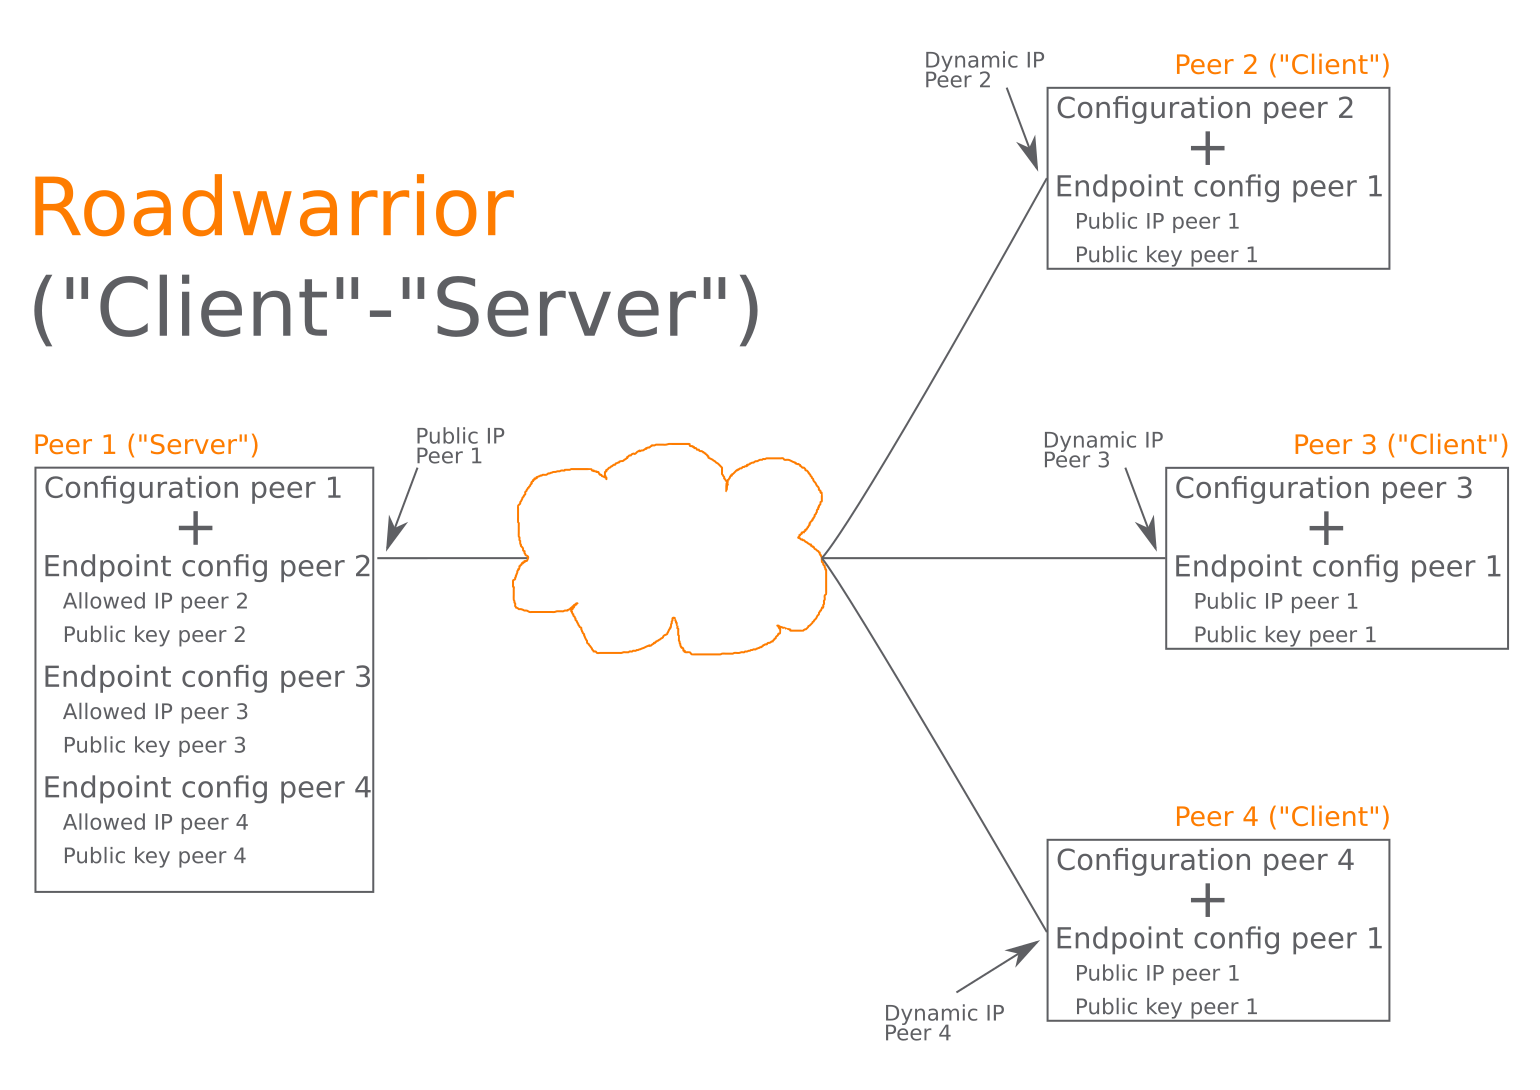
\includegraphics[width=10cm]{figure/Wireguard-roadwarrior.png}
    \caption{Architettura di installazione di WireGuard}
\end{figure}


\subsection{Configurazione del profilo VPN per un client}
Affinché un client possa connettersi alla VPN, è necessario che nel file di configurazione del server sia presente la chiave pubblica del client, e nel profilo di connessione del client sia presente l'IP pubblico del server, la sua chiave pubblica e l'indirizzo IP che il client assumerà.

\section{Configurazione del Firewall}
Nelle policies del firewall, sono state aggiunte delle voci che autorizzano il traffico proveniente dalle interfacce di rete virtuali strongswan0, tun0 e wg0 a navigare su Internet e a comunicare sulla porta 5201 TCP/UDP con la LAN dei server. Questa sarà la porta utilizzata da un servizio di misura delle performance che sarà in esecuzione sul Web Server, iperf3.